\documentclass[problem]{mcs}

\begin{pcomments}
    \pcomment{FP_ran3p_graph}
    \pcomment{by ARM 12/13/13}
\end{pcomments}

\pkeywords{
  random_walk
  conditional_probability
  conditional_expectation
}

\begin{problem}

%\begin{center}
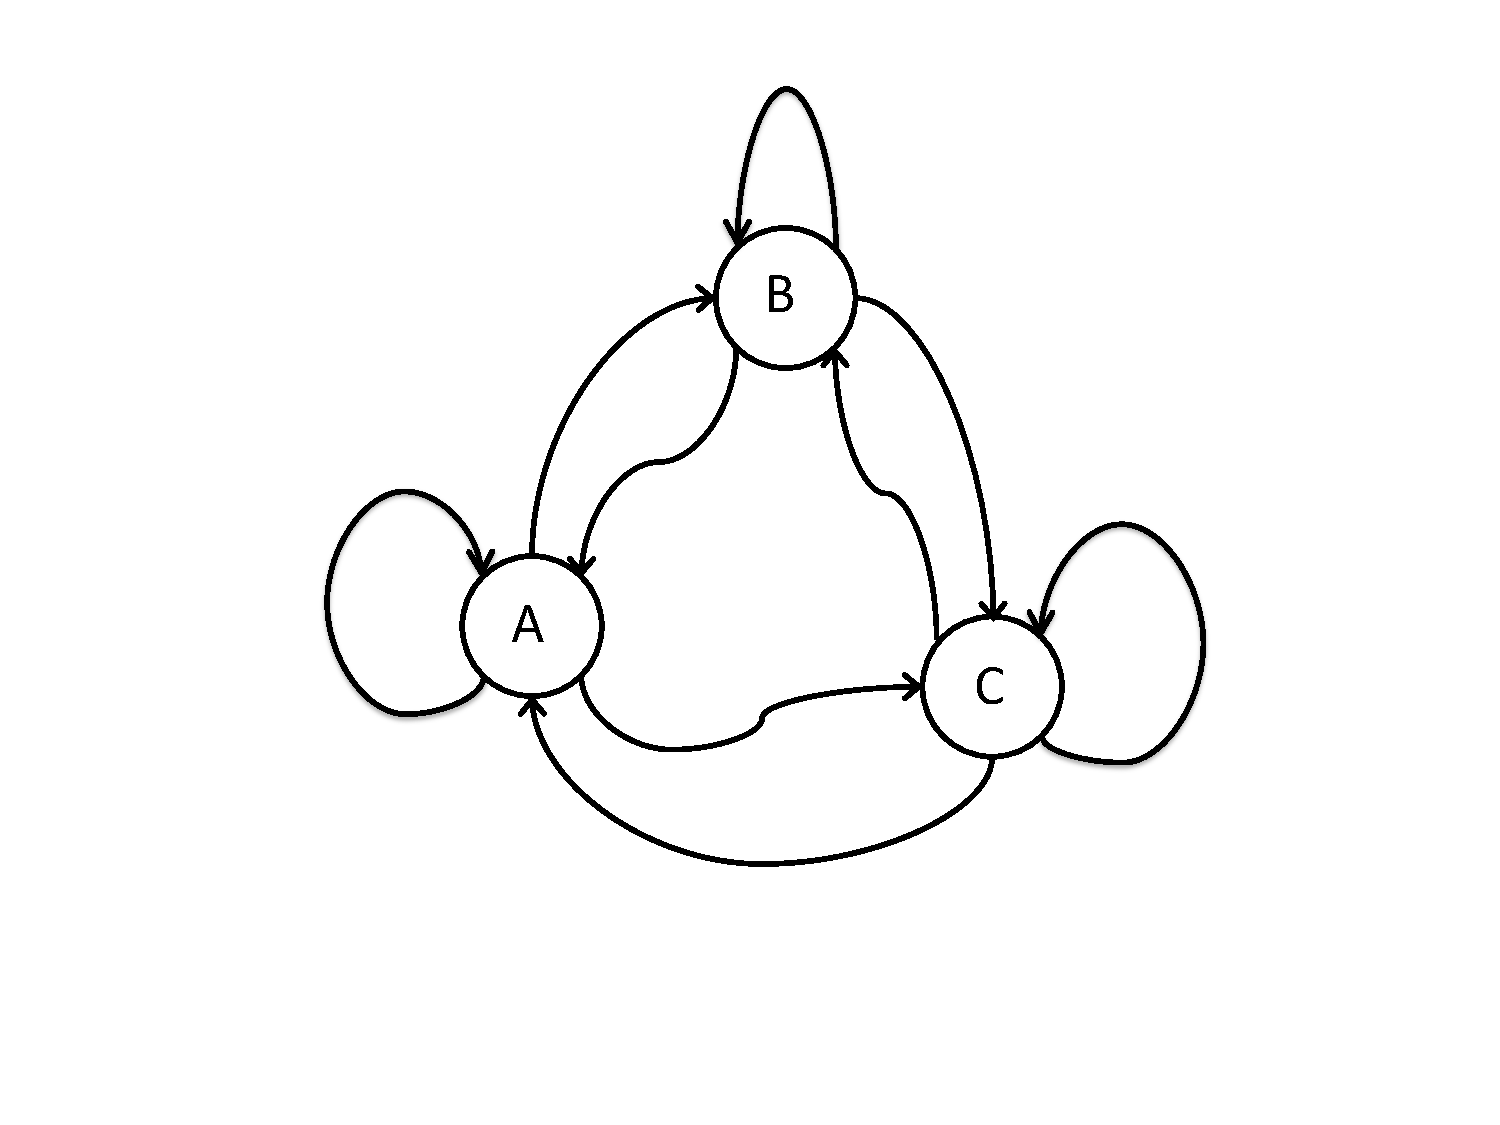
\includegraphics[width=5.0in]{ran-3graph}%{ran-3p-graph}
%\end{center}

The figure above shows a 3-vertex random walk graph (with the edge
probabilities ommited for readability).  For $X,Y \in \set{A,B,C}$,
let $p_{XY}$ denote the probability of the edge $\diredge{X}{Y}$.

Let $a$ be the expected length of a random walk that starts at vertex
$A$ and reaches vertex $C$ for the first time.  Likewise, let $b$ be
the expected length of a random walk that starts at $B$ and reaches
$C$ for the first time.  Write a system of linear equations that can
be solved to yield simple expressions for $a$ and $b$ in terms of
$p_{XY}$'s for $X,Y \in \set{A,B,C}$.  You do \emph{not} need to solve
for $a$ or $b$.

\begin{center}
{\LARGE $a =$} \exambox{3.0in}{0.5in}{-0.1in}
\end{center}

\begin{center}
{\LARGE $b =$} \exambox{3.0in}{0.5in}{0.1in}
\end{center}

\begin{solution}
Let $b$ be the expected length of a random walk that starts at $B$ and
reaches vertex $C$ for the first time.  Then by Conditional
Expectation we have

\begin{align*}
a & = p_{AC}\cdot 1 + p_{AB} \cdot (1 + b) + p_{AA}\cdot (1 + a)\\
b & = p_{BC}\cdot 1 + p_{BA} \cdot (1 + a) + p_{BB}\cdot (1 + b).
\end{align*}

Simplifying (not required) we get
\begin{align*}
a %& = p_{AC}\cdot 1 + p_{AB} \cdot (1 + b) + p_{AA}\cdot (1 + a)\\
  & = p_{AC} + p_{AB} + p_{AB} b + p_{AA} +p_{AA} a\\
  & = p_{AA} a + p_{AB} b + 1,\\
b %& = p_{BC}\cdot 1 + p_{BA} \cdot (1 + a) + p_{BB}\cdot (1 + b)\\
  & = p_{BC} + p_{BA} +  p_{BA} a  + p_{BB} + p_{BB} b\\
  & = p_{BA} a + p_{BB} b + 1.
\end{align*}

\end{solution}

\end{problem}

\endinput
